% !TeX program = lualatex
% !TeX encoding = utf8
% !TeX spellcheck = uk_UA
% !BIB program = bibler

\documentclass{beamer}
\usetheme{Electromagnetism}
\usepackage{Electromagnetism}


%============================================================================
\title[Лекції електрики та магнетизму]{\huge\bfseries Система рівнянь Максвелла}
\subtitle{Лекції з електрики та магнетизму}
\author{Пономаренко С. М.}
\date{}
%============================================================================
\graphicspath{{pictures/}}
\begin{document}
\begin{frame}[plain]
	\maketitle
\end{frame}

% ============================== Слайд ## ===================================
\begin{frame}{Зміст}{}
	\tableofcontents
\end{frame}
% ===========================================================================




% ============================== Слайд ## ===================================
\begin{frame}{Основоположники теорії електромагнітного поля}{}
	\begin{block}{}\justifying
		Теорія електромагнітного поля, початки якої заклав \alert{Фарадей}, математично була завершена \alert{Максвеллом}. При цьому однією з найважливіших
		нових ідей, висунутих Максвеллом, була думка про симетрію в взаємозалежності електричного і магнітного полів.
	\end{block}

	\begin{tblr}{
		colspec={X[c,m]X[c,m]},
		row{2} = {c,m, font=\small}
		}
		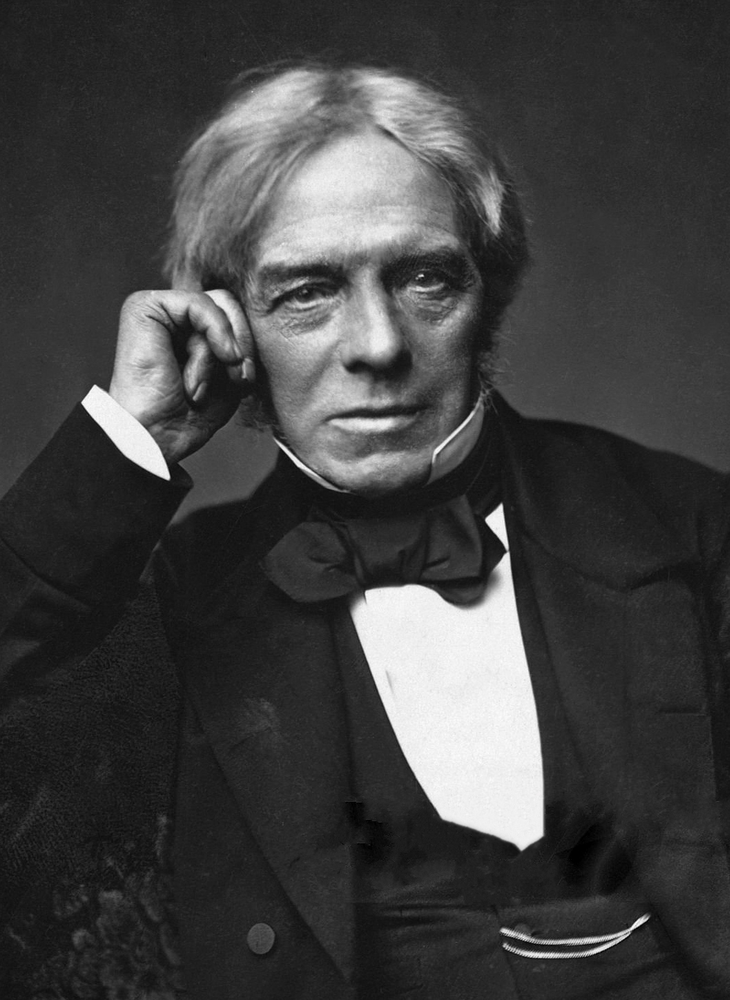
\includegraphics[height=0.75\linewidth]{Faraday} & 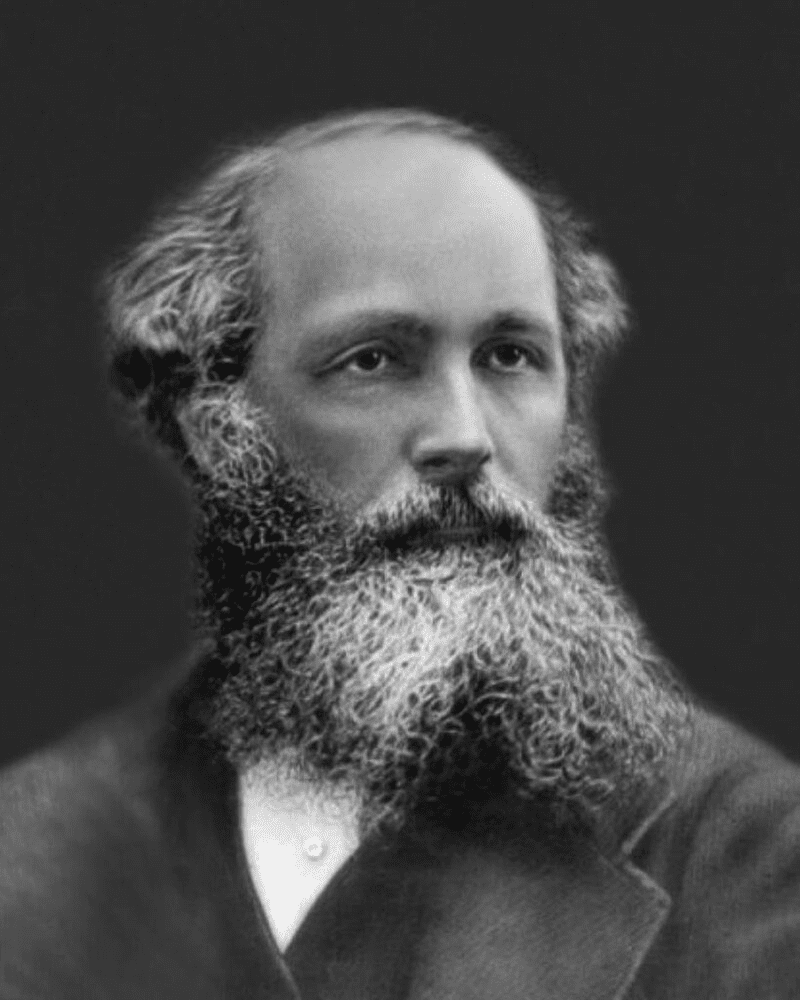
\includegraphics[height=0.75\linewidth]{Maxwell} \\
		\href{https://en.wikipedia.org/wiki/Michael_Faraday}{Майкл Фарадей} (1791 -- 1867) --- англійський фізик і хімік.
		                                                 &
		{\href{https://en.wikipedia.org/wiki/James_Clerk_Maxwell}{Джеймс Клерк Максвелл}\\ (1831 -- 1879) --- шотландський вчений.}
	\end{tblr}
\end{frame}
% ===========================================================================

% ============================== Слайд ## ===================================
\begin{frame}[t]{Цитати із книги <<Еволюція фізики>>}{А. Ейнштейн, Л. Інфельд}
	\tikz[remember picture,overlay] \node[opacity=0.85,inner sep=0pt,
		anchor=south east] at (current page.south east){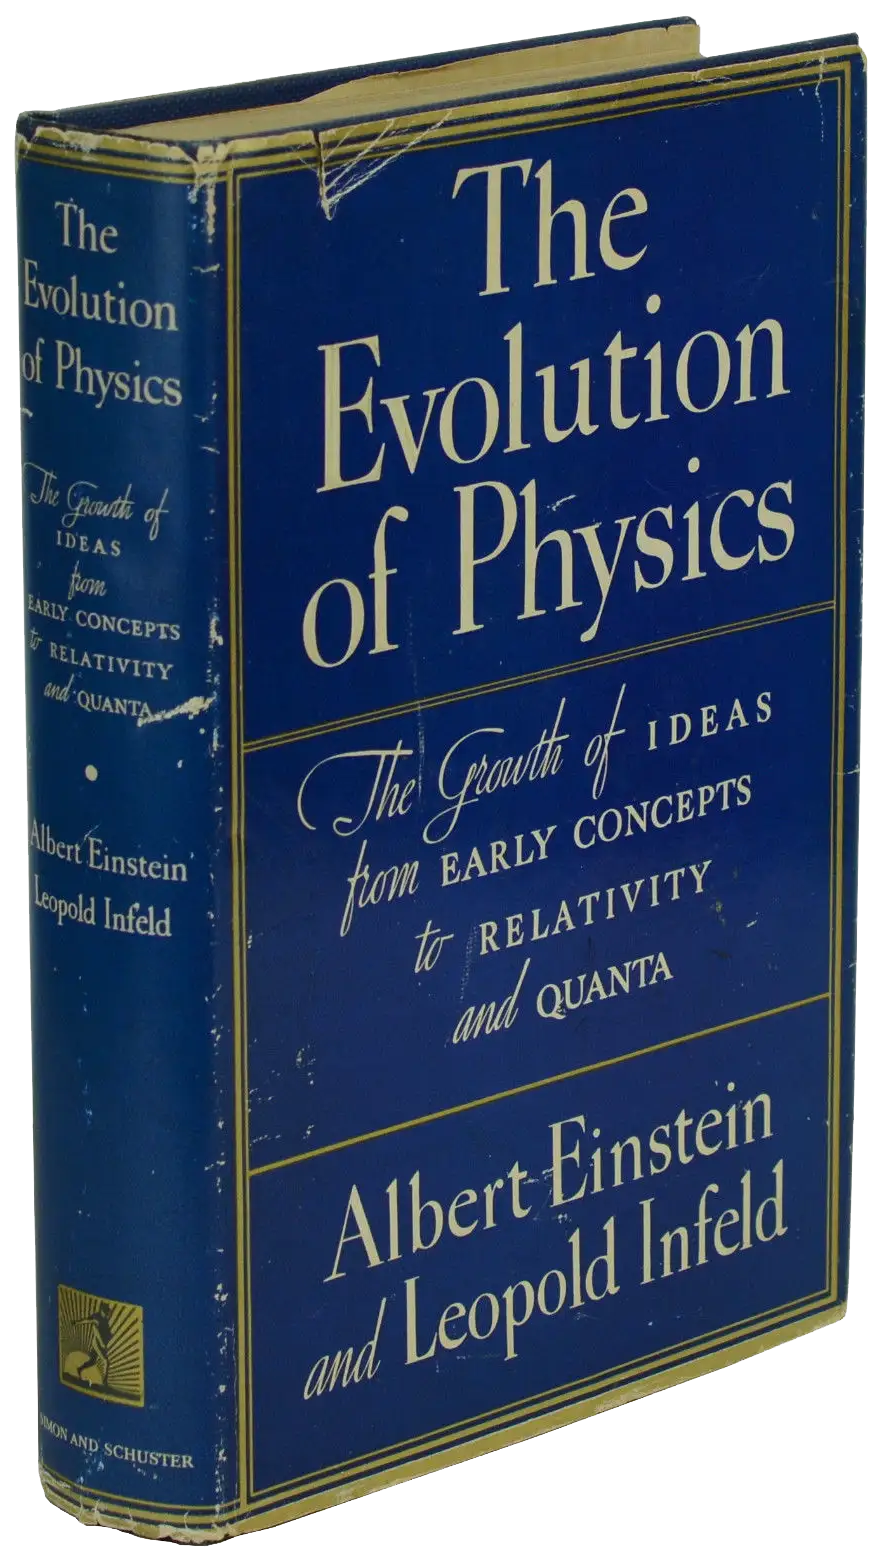
\includegraphics[width=2cm]{Evolution}};
	\begin{block}{}\justifying\itshape
		Кількісне, математичне формулювання законів поля дано в так званих рівняннях Максвелла. \alert{[Експериментальні] факти призвели до формулювання
		цих рівнянь},
		але зміст їх значно багатший [\ldots]. Їхня проста форма приховує глибину, що виявляється тільки при ретельному вивченні.

		\bigskip

		Формулювання цих рівнянь є найважливішою подією з часу Ньютона не тільки важливою подією з часу Ньютона не тільки внаслідок цінності їхнього змісту, а й
		тому, що вони дають зразок нового типу законів. Характерну особливість рівнянь Максвелла, яка проявляється і в усіх інших рівняннях сучасної фізики,
		можна виразити в одному реченні: \alert{рівняння Максвелла суть закони, що виражають структуру поля}.
	\end{block}
\end{frame}
%

%% --------------------------------------------------------
\section{Струм зміщення}
%% --------------------------------------------------------===========================================================================

% ============================== Слайд ## ===================================
\begin{frame}{Струм зміщення і закон збереження заряду}
	\framesubtitle<1>{Протиріччя в законах магнетизму}
	\begin{onlyenv}<1>
		\begin{block}{}\justifying
			Теорема про циркуляцію для постійного магнітного поля:
			\begin{equation*}
				\Rot\Hfield = \frac{4\pi}{c}\vect{j}
			\end{equation*}
			виявляється невірною у випадку змінного електричного поля.

			\bigskip

			Застосовуючи операцію $\Div$ до цього рівняння і
			враховуючи тотожність $\Div\Rot\Hfield = 0$, отримуємо $\Div\vect{j} = 0$. З іншого
			боку, якщо густина заряду змінюється з часом, $\frac{\partial\rho}{\partial t} \neq 0$ то в силу
			закону збереження заряду
			\begin{equation*}
				\Div\vect{j} = - \frac{\partial\rho}{\partial t},
			\end{equation*}
			тобто $\Div\vect{j} \neq 0$. Це протиріччя показує, що необхідно
			видозмінити теорему про циркуляцію.
		\end{block}
	\end{onlyenv}
	\framesubtitle<2>{Гіпотеза Максвелла}
	\begin{onlyenv}<2>
		\begin{block}{}\justifying
			Для вирішення цього протиріччя Дж. Максвелл увів поняття \alert{струму зміщення} $\vect{j}_\text{зм}$ співвідношенням
			\begin{equation*}
				\Rot\Hfield = \frac{4\pi}{c}(\vect{j} + \vect{j}_\text{зм}),
			\end{equation*}
			щоб закон збереження заряду виконувалося. Застосовуючи операцію $\Div$ до записаного рівняння,
			отримуємо:
			\begin{equation*}
				\Div(\vect{j} + \vect{j}_\text{зм}) = 0, \ \Rightarrow\ \Div\vect{j}_\text{зм} = \frac{\partial\rho}{\partial t}.
			\end{equation*}
			За теоремою Гаусса для електричного поля $\rho = \frac1{4\pi}\Div\Dfield$. Отже:
			\begin{equation*}
				\Div\vect{j}_\text{зм} = \frac{\partial}{\partial t}\left( \frac1{4\pi}\Div\Dfield \right),\ \Rightarrow\ \tcbhighmath{\vect{j}_\text{зм} =
					\frac1{4\pi}\frac{\partial\Dfield}{\partial t}.}
			\end{equation*}
		\end{block}
	\end{onlyenv}
	\framesubtitle<3>{Теорема про циркуляцію магнітного поля}
	\begin{onlyenv}<3>
		\begin{block}{}\justifying
			Таким чином, теорема про циркуляцію для магнітного поля,
			що узгоджується із законом збереження заряду, має записуватися у вигляді
			\begin{equation*}
				\tcbhighmath{\Rot\Hfield = \frac{4\pi}{c}\vect{j} + \frac1c\frac{\partial\Dfield}{\partial t},}
			\end{equation*}
			В інтегральній формі теорема про циркуляцію має вигляд
			\begin{equation*}
				\oint\limits_L \Hfield\cdot d\vect{r} = \frac{4\pi}{c} \iint\limits_S\vect{j}\cdot d\vect{S} + \frac1c\iint\limits_S
				\frac{\partial\Dfield}{\partial t} \cdot d\vect{S},
			\end{equation*}
			де $I_\text{зм} =  \frac1{4\pi} \iint\limits_S\frac{\partial\Dfield}{\partial t} \cdot d\vect{S}$ --- струм зміщення, що пронизує площу $S$, натягнуту
			на контур $L$.
			Отже, згідно гіпотези Максвелла \alert{змінне електричне поле поряд зі звичайними струмами, також створює магнітне поле}.
		\end{block}
	\end{onlyenv}%
	\framesubtitle<4>{Порівняння закону Фарадея та гіпотези Максвелла}%
	\begin{onlyenv}<4>
		\begin{block}{}\justifying
			Порівняємо закон електромагнітної індукції Фарадея, та <<оновлену>> теорему про циркуляцію за відсутності струмів провідності ($\vect{j} = 0$) у
			вакуумі ($\epsilon = \mu = 1$ $\Rightarrow$ {\color{red}$\Efield = \Dfield$}, {\color{blue}$\Hfield = \Bfield$}).
			\begin{center}\small
				\begin{tblr}%
					{
					colspec={X[c,m]X[c,m]},
					row{2}={c,m,mode=dmath},
					}
					Закон електромагнітної індукції                          & Закон магнітоелектричної індукції                        \\
					\Rot\Efield = -\frac1c\frac{\partial\Bfield}{\partial t} & \Rot\Bfield = +\frac1c\frac{\partial\Efield}{\partial t} \\
					\tikz[rotate=90, scale=0.9, >=latex, midarrow/.style={%
								postaction={ decorate,
										decoration={ markings, mark=at position .7 with {\arrow{latex}}}}}]{
						\begin{scope}[xshift=0.25cm]
							\draw[arrowpos={0.5}{2pt}{4pt}, red] (1.1,0) [partial ellipse=360:0:0.15 and 0.5];
							\draw[arrowpos={0.5}{2pt}{4pt}, red] (1.1,0) [partial ellipse=360:0:0.3 and 1];
							\draw[arrowpos={0.5}{2pt}{4pt}, red] (1.1,0) [partial ellipse=360:0:0.6 and 2] node[pos=0.5, below] {$\Efield$};
						\end{scope}

						\foreach \y in {-3,...,3}{
								\draw[blue, midarrow] plot[domain=1:3] (\x, 0.2*\y+0.05*\y*\x^2);
							}
						\node[blue, font=\small] at (3.5, 0) {$\frac{\partial\Bfield}{\partial t}>0$};
					}
					                                                         &
					\tikz[rotate=90, scale=0.9, >=latex, midarrow/.style={%
								postaction={ decorate,
										decoration={ markings, mark=at position .7 with {\arrow{latex}}}}}]{
						\begin{scope}[xshift=0.25cm]
							\draw[arrowpos={0.5}{2pt}{4pt}, blue] (1.1,0) [partial ellipse=0:360:0.15 and 0.5];
							\draw[arrowpos={0.5}{2pt}{4pt}, blue] (1.1,0) [partial ellipse=0:360:0.3 and 1];
							\draw[arrowpos={0.5}{2pt}{4pt}, blue] (1.1,0) [partial ellipse=0:360:0.6 and 2] node[pos=0.5, below] {$\Bfield$};
						\end{scope}

						\foreach \y in {-3,...,3}{
								\draw[red, midarrow] plot[domain=1:3] (\x, 0.2*\y+0.05*\y*\x^2);
							}
						\node[red, font=\small] at (3.5, 0) {$\frac{\partial\Efield}{\partial t}>0$};
					}
				\end{tblr}
			\end{center}
		\end{block}
		\begin{alertblock}{}\centering
			Змінне в часі магнітне поле породжує вихрове електричне поле, а змінне в часі електричне поле породжує магнітне поле.
		\end{alertblock}
	\end{onlyenv}
\end{frame}
% ===========================================================================

%% --------------------------------------------------------
\subsection{Приклади розрахунку струмів зміщення}
%% --------------------------------------------------------


% ============================== Слайд ## ===================================
\begin{frame}{Радіальне стікання заряду з кулі}{}\small
	\begin{block}{}\justifying
		Нехай куля несе заряд $Q$, який стікає в зовнішнє середовище. Унаслідок стікання заряду виникають струми, які можуть індукувати магнітне поле.
		Знайдемо це магнітне поле.
	\end{block}
	\begin{columns}
		\begin{column}{0.25\linewidth}\centering
			\begin{tikzpicture}[>=latex]
				\draw[ball color=red!50] (0, 0) circle[radius=0.5cm];
				\draw[dashed] (0, 0) circle[radius=0.75cm];
				\foreach \a in {0,45,...,340}{
						\draw[brown, ->] (0,0) ++(\a:0.75) -- ++(\a:0.25) node[anchor={180+\a}] {$I$};
						\draw[orange, <-] (0,0) ++({\a+45/2}:0.75) -- ++({\a+45/2}:0.25) node[anchor={180+\a+45/2}] {$I_\text{зм}$};
					}
			\end{tikzpicture}
		\end{column}
		\begin{column}{0.75\linewidth}
			\begin{block}{}\justifying
				Стікання заряду з кулі створює струм провідності, який дорівнює:
				\begin{equation*}
					I = -\frac{\partial Q}{\partial t}.
				\end{equation*}
				Електричне поле кулі $\Efield(r) = \frac{Q(t)}{r^3}\vect{r}$ також зменшується з часом, а тому струм зміщення дорівнює:
				\begin{equation*}
					I_\text{зм} = \frac1{4\pi} \oiint\limits_S \frac{\partial\Efield}{\partial t}\cdot d\vect{S} = + \frac{\partial Q}{\partial t} = -I.
				\end{equation*}
			\end{block}
		\end{column}
	\end{columns}
	\begin{block}{}\justifying
		З теореми про циркуляцію:
		\begin{equation*}
			\oint\limits_L \Hfield\cdot d\vect{r} = \frac{4\pi}{c} (I + I_\text{зм}) = 0,\ \Rightarrow\ \Hfield = \Bfield = 0.
		\end{equation*}
	\end{block}
	Отже, в цьому випадку, магнітного поля не виникає.
\end{frame}
% ===========================================================================



% ============================== Слайд ## ===================================
\begin{frame}{Струм зміщення в конденсаторі}{}
	\begin{columns}
		\begin{column}{0.5\linewidth}\centering
			\begin{tblr}{
				colspec={X[c, m]X[c,m]},
				row{2} = {c,m, font=\scriptsize}
				}
                \begin{tikzpicture}[scale=0.6]
					\clip (-1.5, -2.5) rectangle ++(4, 5.5);
					\draw[line width=2pt, gray!50, arrowpos={0.7}{0pt}{7pt}] (0, -2) coordinate (A) -- ++(0, 2);
					\draw[line width=3pt, red!50] (-1, 0) -- (1, 0);
					\draw[line width=2pt, gray!50, arrowpos={0.7}{0pt}{7pt}] (0, 0.5) -- ++(0, 2) coordinate (B);
					\draw[line width=3pt, blue!50] (-1, 0.5) -- (1, 0.5)  ;
					\draw [arrowpos={0.5}{4pt}{4pt}, bend left=120, looseness=2] (B) to (A);
					\draw[fill=red!50, opacity=0.5] (0, -1.5) circle[x radius=1 cm, y radius= 0.3 cm];
					\draw[line width=2pt, gray!50] (0, -1.5) -- ++(0, 0.4);
				\end{tikzpicture}
				 &
				\begin{tikzpicture}[scale=0.6]
					\clip (-1.5, -2.5) rectangle ++(4, 5.5);
					\draw[line width=2pt, gray!50, arrowpos={0.7}{0pt}{7pt}] (0, -2) coordinate (A) -- ++(0, 2);
					\draw[line width=3pt, red!50] (-1, 0) -- (1, 0);
					\draw[line width=2pt, gray!50, arrowpos={0.7}{0pt}{7pt}] (0, 0.5) -- ++(0, 2) coordinate (B);
					\draw[line width=3pt, blue!50] (-1, 0.5) -- (1, 0.5)  ;
					\draw [arrowpos={0.5}{4pt}{4pt}, bend left=120, looseness=2] (B) to (A);
					\draw[fill=red!50, opacity=0.6] (0, -1.5) circle[x radius=1 cm, y radius= 0.3 cm];
					\draw[in=55, out=125, looseness=3.9, fill=red!50, opacity=0.5] (-1, -1.5) to (+1, -1.5) arc[x radius=1 cm, y radius= 0.3 cm, start
							angle=0,
							delta angle=180] --cycle;
				\end{tikzpicture}
				\\
				Площа $S$ пронизується лише струмом провідності
				 &
				Площа $S$ пронизується лише струмом зміщення
			\end{tblr}
		\end{column}
		\begin{column}{0.5\linewidth}
			\begin{block}{}\justifying
				Теорема про циркуляцію має вигляд:
				\begin{itemize}
					\item Для лівого рисунка
					      \begin{equation*}
						      \oint\limits_L \Hfield\cdot d\vect{r} = \frac{4\pi}{c}I.
					      \end{equation*}
					\item Для правого рисунка
					      \begin{equation*}
						      \oint\limits_L \Hfield\cdot d\vect{r} = \frac{4\pi}{c}I_\text{зм}.
					      \end{equation*}
				\end{itemize}
			\end{block}
		\end{column}
	\end{columns}
	\begin{overprint}
		\onslide<1>
		\begin{block}{}\justifying\small
			Оскільки різні поверхні спираються на один і той же контур $L$, то циркуляція $\oint\limits_L \Hfield\cdot d\vect{r}$ не повинна залежати вибору
			поверхні. А, отже, $I = I_\text{зм}$, тобто в середині конденсатора <<протікає>> струм зміщення, який замикає коло.
		\end{block}
		\onslide<2>
		\begin{block}{}\justifying\small
			Як видно з теореми про циркуляцію, \alert{струми зміщення} замикають струми провідності і \alert{створюють магнітне поле точно так само}, як і
			струми провідності. Вони, однак, не створюють прямо теплового ефекту, до них незастосовні закон Ома і закон Джоуля-Ленца.
		\end{block}
	\end{overprint}
\end{frame}
% ===========================================================================

%% --------------------------------------------------------
\section{Система рівнянь Максвелла}
%% --------------------------------------------------------

% ============================== Слайд ## ===================================
\begin{frame}{Система рівнянь Максвелла}{}
	\begin{block}{}\justifying\small
		Доповнивши основні факти зі сфери електромагнетизму, та доповнивши їх гіпотезою струмів зміщення, Максвелл зміг написати систему фундаментальних
		рівнянь електродинаміки. Таких рівнянь чотири.
	\end{block}
	\begin{center}
		\begin{tblr}%
			{
			colspec={|Q[l,m, 2.5cm, bg=yellow!10, font=\small]|[1pt, white]X[l,m, bg=red!10]|[1pt, white]Q[l,m, 2.5cm, bg=blue!10]|},
			row{1}={c, fg=white, bg=cyan, font=\bfseries\small},
			cell{2-5}{2-Z}={l, m, mode=dmath, font=\small},
			%hlines,
			}
			\hline
			Рівняння                                                                 & Інтегральна форма                                                                       & Диференціальна форма \\
			\hline\hline
			Теорема Гаусса для магнітного поля                                       & \oiint\limits_S \Bfield\cdot d\vect{S} =  0                                             & \Div\Bfield = 0      \\
			\hline
			Теорема про циркуляцію для електричного поля                             & \oint\limits_L \Efield\cdot d\vect{r} = -
			\frac1c\iint\limits_S \frac{\partial\Bfield}{\partial t} \cdot d\vect{S} & \Rot\Efield = - \frac1c \frac{\partial\Bfield}{\partial t}                                                     \\
			\hline\hline
			Теорема Гаусса для електричного поля                                     & \oiint\limits_S \Dfield\cdot d\vect{S} = 4\pi \iiint\limits_{V} \rho dV                 & \Div\Dfield =
			4\pi\rho                                                                                                                                                                                  \\
			\hline
			Теорема про циркуляцію для магнітного поля                               & \oint\limits_L \Hfield\cdot d\vect{r} = \frac{4\pi}{c} \iint\limits_S \left( \vect{j} +
			\frac1{4\pi}\frac{\partial\Dfield}{\partial t} \right) \cdot d\vect{S}   & \Rot\Hfield = \frac{4\pi}{c}\vect{j} + \frac1c
			\frac{\partial\Dfield}{\partial
				t}
			\\
			\hline
		\end{tblr}
	\end{center}
\end{frame}
% ===========================================================================


% ============================== Слайд ## ===================================
\begin{frame}{Вираз електричного поля через потенціали}{}
	\renewcommand{\baselinestretch}{0.99}
	\begin{block}{}\justifying
		Рівняння Максвелла групуються парами. \alert{Перша пара рівнянь} --- рівняння \alert{без зарядів та струмів}, \alert{друга пара} --- рівняння
		\alert{із зарядами та струмами}.
	\end{block}
	\begin{block}{}
		Теорема Гаусса для магнітного поля дозволяє ввести векторний потенціал:
		\begin{equation*}
			\Bfield=\Rot\vect{A}
		\end{equation*}
		Тоді теорема про циркуляцію для електричного поля записується як:
		\begin{equation*}
			\Rot\left(\Efield  + \frac{\partial\vect{A}}{\partial t}\right) = 0
		\end{equation*}
		Ця рівність означає, що це
		поле може бути представлене як градієнт скалярної функції, тоді отримуємо:
		\begin{equation*}
			\Efield = -\vect{\nabla}\phi - \frac{\partial\vect{A}}{\partial t}
		\end{equation*}
		У випадку постійних у часі полів: $\Efield = -\vect{\nabla}\phi $, тобто, що введена тут функція $\phi$
		збігається зі скалярним потенціалом.
	\end{block}
\end{frame}
% ===========================================================================


% ============================== Слайд ## ===================================
\begin{frame}{Стаціонарні поля}{}
	\begin{block}{}\justifying
		У стаціонарному випадку часткові похідні за часом від полів дорівнюють нулю, тому рівняння максвела розпадається на дві окремі
		системи для електростатики і магнітостатики.
	\end{block}
	\begin{center}
		\begin{tblr}%
			{
			colspec={|X[l,m, bg=yellow!10, font=\scriptsize]|[1pt, white]X[c,m, bg=red!10]|},
			row{1}={c, fg=white, bg=cyan, font=\bfseries},
			cell{2-5}{1-Z}={c, m, mode=dmath, font=},
			%hlines,
			}
			\hline
			Рівняння електростатики & Рівняння магнітостатики \\
			\hline
			\begin{cases}
				\Div\Dfield = 4\pi\rho, \\
				\Rot\Efield = 0.
			\end{cases}
			                        &
			\begin{cases}
				\Div\Bfield = 0, \\
				\Rot\Hfield = \frac{4\pi}{c} \vect{j}.
			\end{cases}
			\\
			\hline
		\end{tblr}
	\end{center}
\end{frame}
% ===========================================================================




% ============================== Слайд ## ===================================
\begin{frame}{Матеріальні рівняння}{}\small
	\begin{block}{}\justifying
		Рівняння Максвелла мають бути доповнені співвідношеннями, що зв'язують поля $\Dfield$ та $\Efield$ з одного боку, та $\Hfield$ та $\Bfield$ з
		іншого
		боку.
	\end{block}
	\begin{center}
		\begin{tblr}%
			{
			colspec={|X[l,m, bg=yellow!10, font=\small]|[1pt, white]Q[l,m, 0.2\linewidth,bg=red!10]|},
			row{1}={c, fg=white, bg=cyan, font=\bfseries},
			cell{2-Z}{2-Z}={l, m, mode=dmath, font=\small},
			hlines,
			}
			                                                                                           & Вираз                            \\
			Вектор індукції електричного поля                                                          & \Dfield = \Efield + 4\pi\vect{P} \\
			Вектор поляризації (для лінійних ізотропних речовин)                                       & \vect{P} = \chi_e\Efield         \\
			Діелектрична проникніть  (для лінійних ізотропних речовин)                                 & \epsilon = 1 + 4\pi \chi_e       \\
			Зв'язок $\Dfield$ та $\Efield$ (для лінійних ізотропних речовин)                           & \Dfield = \epsilon\Efield        \\
			\hline
			Вектор напруженості магнітного поля                                                        & \Hfield = \Bfield - 4\pi\vect{J} \\
			Вектор намагнічування (для лінійних ізотропних речовин)                                    & \vect{J} = \chi_e\Hfield         \\
			Магнітна проникніть  (для лінійних ізотропних речовин)                                     & \mu = 1 + 4\pi \chi_m            \\
			Зв'язок $\Hfield$ та $\Bfield$ (для лінійних ізотропних речовин)                           & \Bfield = \mu\Hfield             \\
			\hline
			У разі струму, спричиненого електричним полем у провідному середовищі, має місце закон Ома & \vect{j} = \lambda\Efield
		\end{tblr}
	\end{center}
\end{frame}
% ===========================================================================



% ============================== Слайд ## ===================================
\begin{frame}{Граничні умови}{}\small
	\begin{block}{}\justifying
		Диференціальні рівняння Максвелла треба доповнити граничними умовами, яким має задовольняти електромагнітне поле на межі
		розділу двох середовищ. Ці умови неявно містяться в інтегральній формі рівнянь Максвелла і отримуються за їх допомогою. Граничні умови в стаціонарному
		випадку аналогічні і для випадку змінних полів.
	\end{block}
	\begin{center}
		\begin{tblr}%
			{
			colspec={|X[l,m, bg=yellow!10, font=\small]|[1pt, white]X[c,m, bg=red!10]|},
			row{1}={c, fg=white, bg=cyan, font=\bfseries},
			cell{2-Z}{1-Z}={c, m, mode=dmath, font=},
			%hlines,
			}
			\hline
			Умови для електричних векторів & Умови для магнітних векторів \\
			\hline
			D_{2n} - D_{1n} = 4\pi\sigma
			                               &
			B_{1n} = B_{2n}
			\\
			\hline
			\hline
			E_{1\tau} = E_{2\tau}
			                               &
			\left[\vect{n}\times\Hfield_2\right] - \left[\vect{n}\times\Hfield_1\right] = \frac{4\pi}{c}\vect{i}
			\\
			\hline
		\end{tblr}
	\end{center}
	\begin{block}{}\justifying
		Тут $\sigma$ ---  поверхнева густина вільних електричних зарядів, a $\vect{i}$ --- поверхнева густина струму провідності на розглянутій границі
		розділу. У випадку, коли поверхневих струмів немає, гранична умова для тангенціальної компоненти вектора напруженості магнітного поля набуває
		вигляду:
		\begin{equation*}
			H_{1\tau} = H_{2\tau}
		\end{equation*}
	\end{block}
\end{frame}
% ===========================================================================


%% --------------------------------------------------------
\section{Енергія електромагнітного поля}
%% --------------------------------------------------------


% ============================== Слайд ## ===================================
\begin{frame}{Закон збереження енергії електромагнітного поля}{}
	\begin{columns}
		\begin{column}{0.4\linewidth}\centering
			\begin{tikzpicture}[>=latex, scale=0.75]
				\pgfmathsetseed{55}
				\foreach \a in {0,10,...,350}
					{
						\pgfmathparse{1.2*abs(rand)}
						\node[inner sep=1pt, circle, ball color=red!50] at (\a:{\pgfmathresult}) {};
						\draw[->] (0,0) ++(\a:2) -- ++(\a:0.5);
					}
				\draw[ball color=gray!5, name path=metall, smooth, opacity=0.5] plot
					[smooth cycle,
						samples=8,domain={1:10}]
				(\x*360/10+5*rnd:1cm+1cm*rnd);
			\end{tikzpicture}
		\end{column}
		\begin{column}{0.6\linewidth}
			\begin{block}{}\justifying
				Якщо  у деякій області простору присутнє електромагнітне поле та заряджені частинки, які взаємодіють з цим полем, то енергія такої
				системи має
				зберігатись, якщо система замкнена. Якщо ж система незамкнена, то енергія може як втікати в цю область, так і витікати з неї.
			\end{block}
		\end{column}
	\end{columns}
	\begin{block}{}\centering\small
		(Зміна енергії в об'ємі) = (Рух частинок) + (Потік енергії на зовні).
	\end{block}

	\begin{block}{}\centering\small
		(Рух частинок) = (Зміна енергії в об'ємі) -- (Потік енергії на зовні).
	\end{block}

	\begin{block}{}
		Рухати частинки може лише електричне поле. Енергія, яка витрачається полем на розгін частинок в одиниці об'єму за одиницю часу ---
		джоулеве тепло
		$\vect{j}\cdot\Efield$.
	\end{block}
\end{frame}
% ===========================================================================




% ============================== Слайд ## ===================================
\begin{frame}{Закон збереження енергії електромагнітного поля}{}
	\begin{columns}
		\begin{column}{0.4\linewidth}\centering
			\begin{tikzpicture}[>=latex, scale=0.75]
				\pgfmathsetseed{55}
				\foreach \a in {0,10,...,350}
					{
						\pgfmathparse{1.2*abs(rand)}
						\node[inner sep=1pt, circle, ball color=red!50] at (\a:{\pgfmathresult}) {};
						\draw[->] (0,0) ++(\a:2) -- ++(\a:0.5);
					}
				\draw[ball color=gray!5, name path=metall, smooth, opacity=0.5] plot
					[smooth cycle,
						samples=8,domain={1:10}]
				(\x*360/10+5*rnd:1cm+1cm*rnd);
			\end{tikzpicture}
		\end{column}
		\begin{column}{0.6\linewidth}
			\begin{block}{}\justifying
				Якщо  у деякій області простору присутнє електромагнітне поле та заряджені частинки, які взаємодіють з цим полем, то енергія
				такої системи має
				зберігатись, якщо система замкнена. Якщо ж система незамкнена, то енергія може як втікати в цю область, так і витікати з неї.
			\end{block}
		\end{column}
	\end{columns}
	\begin{block}{}\centering\small
		(Зміна енергії в об'ємі) = (Рух частинок) + (Потік енергії на зовні).
	\end{block}

	\begin{block}{}\centering\small
		(Рух частинок) = (Зміна енергії в об'ємі) -- (Потік енергії на зовні).
	\end{block}

	\begin{block}{}
		Рухати частинки може лише електричне поле. Енергія, яка витрачається полем на розгін частинок в одиниці об'єму за одиницю часу ---
		джоулеве тепло $\vect{j}\cdot\Efield$.
	\end{block}
\end{frame}
% ===========================================================================



% ============================== Слайд ## ===================================
\begin{frame}{Отримання закону збереження}{}\small
	\begin{block}{}
		\begin{equation*}
			\vect{j} = \frac{c}{4\pi} \Rot\Hfield - \frac1c \parttime{\Dfield}, \quad \text{(рівняння Максвелла для $\Rot\Hfield$)}.
		\end{equation*}
		\begin{equation*}
			\vect{j}\Efield =  \frac{c}{4\pi}\Efield\cdot\Rot\Hfield - \frac1{4\pi}\Efield\cdot\frac{\partial\Dfield}{\partial t}
		\end{equation*}
		\begin{equation*}
			\Efield\cdot\Rot\Hfield  = - \Div[\Efield\times\Hfield] + \Hfield\cdot\Rot\Efield, \quad \text{(формула векторного аналізу)}.
		\end{equation*}
		\begin{equation*}
			\vect{j}\cdot\vect{E} =  - \Div\left(\frac{c}{4\pi}[\Efield\times\Hfield]\right) + \frac{c}{4\pi}  \Hfield\cdot \Rot\Efield  -
			\parttime{}
			\left( \frac1{8\pi}\epsilon\Efield^2\right)
		\end{equation*}

		\begin{equation*}
			\Rot\Efield = - \frac1c \parttime{\Bfield}, \quad \text{(рівняння Максвелла для $\Rot\Efield$)}.
		\end{equation*}
		Врахуємо матеріальні рівняння $\Dfield = \epsilon\Efield$ та $\Bfield = \mu\Hfield$.
		\begin{equation*}
			\vect{j}\cdot\vect{E} =  - \Div\left(\frac{c}{4\pi}[\Efield\times\Hfield]\right) - \frac{1}{4\pi}  \Hfield\cdot
			\parttime{\Bfield}  -
			\parttime{} \left( \frac1{8\pi}\epsilon\Efield^2\right)
		\end{equation*}

		\begin{equation*}
			\vect{j}\cdot\vect{E} =  - \Div\left(\frac{c}{4\pi}[\Efield\times\Hfield]\right) -  \parttime{} \left(
			\frac1{8\pi}\epsilon\Efield^2 +
			\frac1{8\pi}\mu\Hfield^2 \right)
		\end{equation*}

	\end{block}
\end{frame}
% ===========================================================================


%% --------------------------------------------------------
\subsection{Теорема Пойнтінга}
%% --------------------------------------------------------


% ============================== Слайд ## ===================================
\begin{frame}{Теорема Пойнтінга}{}\small
	\begin{onlyenv}<1>
		\begin{block}{}\justifying
			Проаналізуємо отриманий вираз:
			\begin{equation*}
				\underbrace{\vect{j}\cdot\vect{E}}_\text{Енергія руху частинок} =  -
				\Div\underbrace{\left(\frac{c}{4\pi}[\Efield\times\Hfield]\right)}_\text{Вектор $\vect{\Pi}$} -  \parttime{}
				\underbrace{\left( \frac{\epsilon\Efield^2}{8\pi} + \frac{\mu\Hfield^2}{8\pi}
					\right)}_\text{\parbox{3.5cm}{\centering\scriptsize\strut\ignorespaces Густина
						енергії\\ електромагнітного поля $w$}}
			\end{equation*}
		\end{block}
	\end{onlyenv}
	\begin{onlyenv}<1-2>
		\begin{block}{}
			Закон збереження енергії
		\end{block}
		\begin{columns}
			\begin{column}{0.4\linewidth}
				\begin{equation*}
					\tcbhighmath{-\parttime{w} = \Div\vect{\Pi} + \vect{j}\cdot\vect{E}}
				\end{equation*}
			\end{column}
			\begin{column}{0.6\linewidth}
				\begin{equation*}
					\tcbhighmath{-\parttime{W} = \oiint\limits_S\vect{\Pi}\cdot d\vect{S} + \iiint\limits_V \vect{j}\cdot\vect{E} dV}
				\end{equation*}
			\end{column}
		\end{columns}
		\begin{block}{Теорема Пойнтінга}\justifying
			Зменшення енергії за одиницю часу в даному об'ємі дорівнює потоку енергії крізь поверхню, обмежену цим об'ємом, плюс потужність
			$Р$, яку сили поля виконують над зарядами речовини всередині даного об'єму.
		\end{block}
	\end{onlyenv}
	\begin{onlyenv}<2>
		\begin{block}{Вектор Пойнтінга}\justifying
			\begin{equation*}
				\tcbhighmath{\vect{\Pi} = \frac{c}{4\pi}[\Efield\times\Hfield]}
			\end{equation*}
			Вектор визначає кількість енергії поля, що протікає через одиничну площадку в одиницю часу, і показує напрямок руху енергії
			електромагнітного поля.
		\end{block}
	\end{onlyenv}
\end{frame}
% ===========================================================================



% ============================== Слайд ## ===================================
\begin{frame}{Одиниці вимірювання величин}{}
	Вектор густини потоку енергії (вектор Пойнтінга)
	\begin{equation*}
		\vect{\Pi} = \frac{c}{4\pi}[\Efield\times\Hfield], \quad [\Pi] = \frac{\text{ерг}}{\text{см}^2 \cdot \text{с}}\, (\text{СГС}),\ [S] =
		\frac{\text{Вт}}{\text{м}^2}\, (\text{SI})
	\end{equation*}

	Густина енергії
	\begin{equation*}
		w = \frac{\Efield\cdot\Dfield}{8\pi} + \frac{\Bfield\cdot\Hfield}{8\pi}, \quad [w] = \frac{\text{ерг}}{\text{см}^2}\, (\text{СГС}),\
		[w] = \frac{\text{Дж}}{\text{м}^3}\, (\text{SI})
	\end{equation*}
\end{frame}
% ===========================================================================


%% --------------------------------------------------------
\subsection{Приклади використання теореми Пойнтінга}
%% --------------------------------------------------------


% ============================== Слайд ## ===================================
\begin{frame}{Зарядка конденсатора}{}\small
	\begin{columns}
		\begin{column}{0.35\linewidth}\centering
			\begin{tikzpicture}[scale=0.8, >=latex, midarrow/.style={%
							postaction={ decorate,
									decoration={ markings, mark=at position .8 with {\arrow{latex}}}}}]{
					\draw[blue] (0,0) circle(0.5 and 0.15);
					\draw[blue] (0,0) circle(1 and 0.3);
					\draw[blue] (0,0) circle(2 and 0.6);

					\foreach \x in {-2,-1,...,2}{
							\draw[red, midarrow] (\x, -1.5) -- (\x, 1.5);
						}
				}
				\draw[blue, arrowpos={0.5}{2pt}{4pt}] (0,0) ++(180:0.5) arc(180:360:0.5 and 0.15);
				\draw[blue, arrowpos={0.5}{2pt}{4pt}] (0,0) ++(180:1) arc(180:360:1 and 0.3);
				\draw[blue, arrowpos={0.5}{2pt}{4pt}] (0,0) ++(180:2) arc(180:360:2 and 0.6);

				\draw[line width=2pt, blue!50] (-2.5, 1.5) -- (2.5, 1.5);
				\draw[line width=2pt, red!50] (-2.5, -1.5) -- (2.5, -1.5);

				\draw [blue, ->] (0:2) coordinate (S) -- ++(70:0.5) node[right] {$\Hfield$};
				\node[left, red] at (2, 1) {$\Efield$};
				\draw [orange!60!black, ->] (S) -- ++(-0.75,0) node[below] {$\vect{\Pi}$};
			\end{tikzpicture}

		\end{column}
		\begin{column}{0.65\linewidth}
			\begin{overprint}
				\onslide<1>
				\begin{block}{}\justifying
					Плоский конденсатор із пластинами радіуса \( R \) заряджається струмом \( I \) від зовнішнього джерела енергії . Якщо в
					деякий момент
					заряд на нижній пластині дорівнює \( q \), то індукція поля всередині конденсатора дорівнює:
					\(
					D = 4 \pi \sigma = \frac{4 \pi q}{\pi R^2},
					\)
					і напрямлений від нижньої пластини до верхньої.
					Густина струму зміщення в конденсаторі:
					\(
					j_{\text{зм}} = \frac{\dot{D}}{4 \pi} = \frac{\dot{q}}{\pi R^2}.
					\)
				\end{block}
				\onslide<2-3>
				\begin{block}{}\justifying
					Вектор Пойнтінга
					\(
					\vect{\Pi} = \frac{c}{4\pi}\left[\Efield\times\Hfield\right]
					\)
					спрямований до осі конденсатора і дорівнює за величиною на межі (\( r = R \)):
					\[
						\Pi = \frac{c}{4 \pi} EH = \frac{c}{4 \pi} \left( \frac{4 \pi q}{\varepsilon \pi R^2} \right) \left( \frac{2
							\dot{q}}{c R}
						\right) =
						\frac{1}{\varepsilon
							\pi R^2} 2 q \dot{q}.
					\]
				\end{block}
			\end{overprint}
		\end{column}
	\end{columns}
	\begin{overprint}
		\onslide<1-2>
		\begin{block}{}\justifying
			Цей струм породжує в конденсаторі магнітне поле, яке можна знайти за допомогою теореми про циркуляцію:
			\[
				\oint\limits_{L} \mathbf{H} \, d\mathbf{r} = \frac{4 \pi}{c} J_{\text{зм}}(r)
				\Rightarrow 2 \pi r H(r) = \frac{4 \pi}{c} \pi r^2 j_{\text{зм}}(r)
				\Rightarrow H(r) = \frac{2r}{c R^2} \dot{q}.
			\]

			Тут за контур \( L \) узято коло радіусу \( r \) з центром на осі конденсатора. Маючи на увазі, що конденсатор заряджається (\(
			\dot{q} > 0 \)), робимо висновок, що струм зміщення спрямований від нижньої пластини до верхньої. Це означає, що силові лінії
			магнітного поля
			спрямовані, як 	показано на рис.
		\end{block}
		\onslide<3>
		\begin{block}{}\justifying
			Якщо відстань між пластинами дорівнює \( h \), то енергія, що втікає в конденсатор за одиницю часу, дорівнює:
			\[
				\frac{dW}{dt} = S \cdot 2 \pi R h = \frac{1}{\varepsilon \pi R^2} \cdot q \dot{q} \cdot 2 \pi R h = \frac{q \dot{q}}{C},
			\]
			де \( C = \epsilon \pi R^2 / 4\pi h\) --- ємність конденсатора. За кінцевий час, при досягненні заряду q на пластині, енергія складе:
			\[
				W = \frac{q^2}{2C}.
			\]
			Ми прийшли до відомої формули для енергії, що запасається в конденсаторі.
		\end{block}
	\end{overprint}
\end{frame}
% ===========================================================================



% ============================== Слайд ## ===================================
\begin{frame}{Довгий провідник}{}\small
	\begin{columns}
		\begin{column}{0.3\linewidth}\centering
			\begin{tikzpicture}[>=latex]
				\draw[fill=gray!50] (0, 0) -- ++(0,2) arc(180:360:1 and 0.3) -- ++(0, -2) arc(0:-180:1 and 0.3);
				\draw[fill=gray!50] (1, 2) circle (1 and 0.3);
				\draw[blue, arrowpos={0.5}{2pt}{4pt}] (1, 1) [partial ellipse=155:385:1.1 and 0.3] node[pos=0.5, below] {$\Hfield$};
				\draw[->, red] (1, 1) -- ++(0, 0.5) node[left] {$\Efield$};
				\draw[->, orange!60!black, thick] (2.1, 1) -- ++(-0.5, 0) node[above] {$\vect{\Pi}$};
			\end{tikzpicture}
		\end{column}
		\begin{column}{0.7\linewidth}
			\begin{block}{}\justifying
				Розглянемо довгий прямий дріт радіуса $R$ і довжини $\ell$, яким тече струм $I$ . На зовнішній поверхні дроту
				присутнє магнітне поле $H = \frac{2I}{cR}$. Струм у дроті виникає
				завдяки напрузі $U$ на його кінцях, що створює поле величиною $E = \frac{U}{\ell}$. Напрямки полів $\Efield$ і $\Hfield$
				показано на рис.
			\end{block}
		\end{column}
	\end{columns}
	\begin{block}{}\justifying
		Вектор Пойнтінга виявляється спрямованим до осі дроту і дорівнює за величиною:
		\begin{equation*}
			\Pi = \frac{c}{4\pi} EH = \frac{c}{4\pi} \frac{U}{\ell} \frac{2I}{cR} = \frac{1}{2\pi\ell R} UI
		\end{equation*}
		Оскільки площа бічної поверхні дроту дорівнює $S= 2\pi\ell R$, то повний потік енергії, що втікає в дріт, становить $\Pi S = UI$. Це
		в точності та сама
		енергія, що йде на джоулеві втрати в дроті: $\Pi S = Q = UI$.
	\end{block}
	\begin{block}{}\justifying
		Таким чином, електрони отримують свою енергію, ззовні, від потоку енергії зовнішнього поля всередину дроту і витрачають її на
		створення теплоти. Енергія віддалених зарядів якимось чином розтікається по великій області простору і потім втікає всередину дроту.
	\end{block}
\end{frame}
% ===========================================================================





\end{document}
